\chapter{Localization System Implementation}

\label{Chapter4}

In order to develop and evaluate the system outlined in Chapter \ref{Chapter3}, it is first required to establish a testing environment.
This chapter introduces the implementation of the localization system in a test bed.

\section{System Overview}

The test bed consists of multiple anchor nodes, a mobile node and a computer.

The ANs are commercial WiFi access pints, which are placed in the area of interest and constantly broadcast a beacon signal.

The MN, an android smartphone, is used to collect samples form different location in the area of interest. 

The collected samples are transferred to the computer where the calculations and algorithms for training, testing and evaluating the system can be executed.

\begin{figure}[ht]
\centering
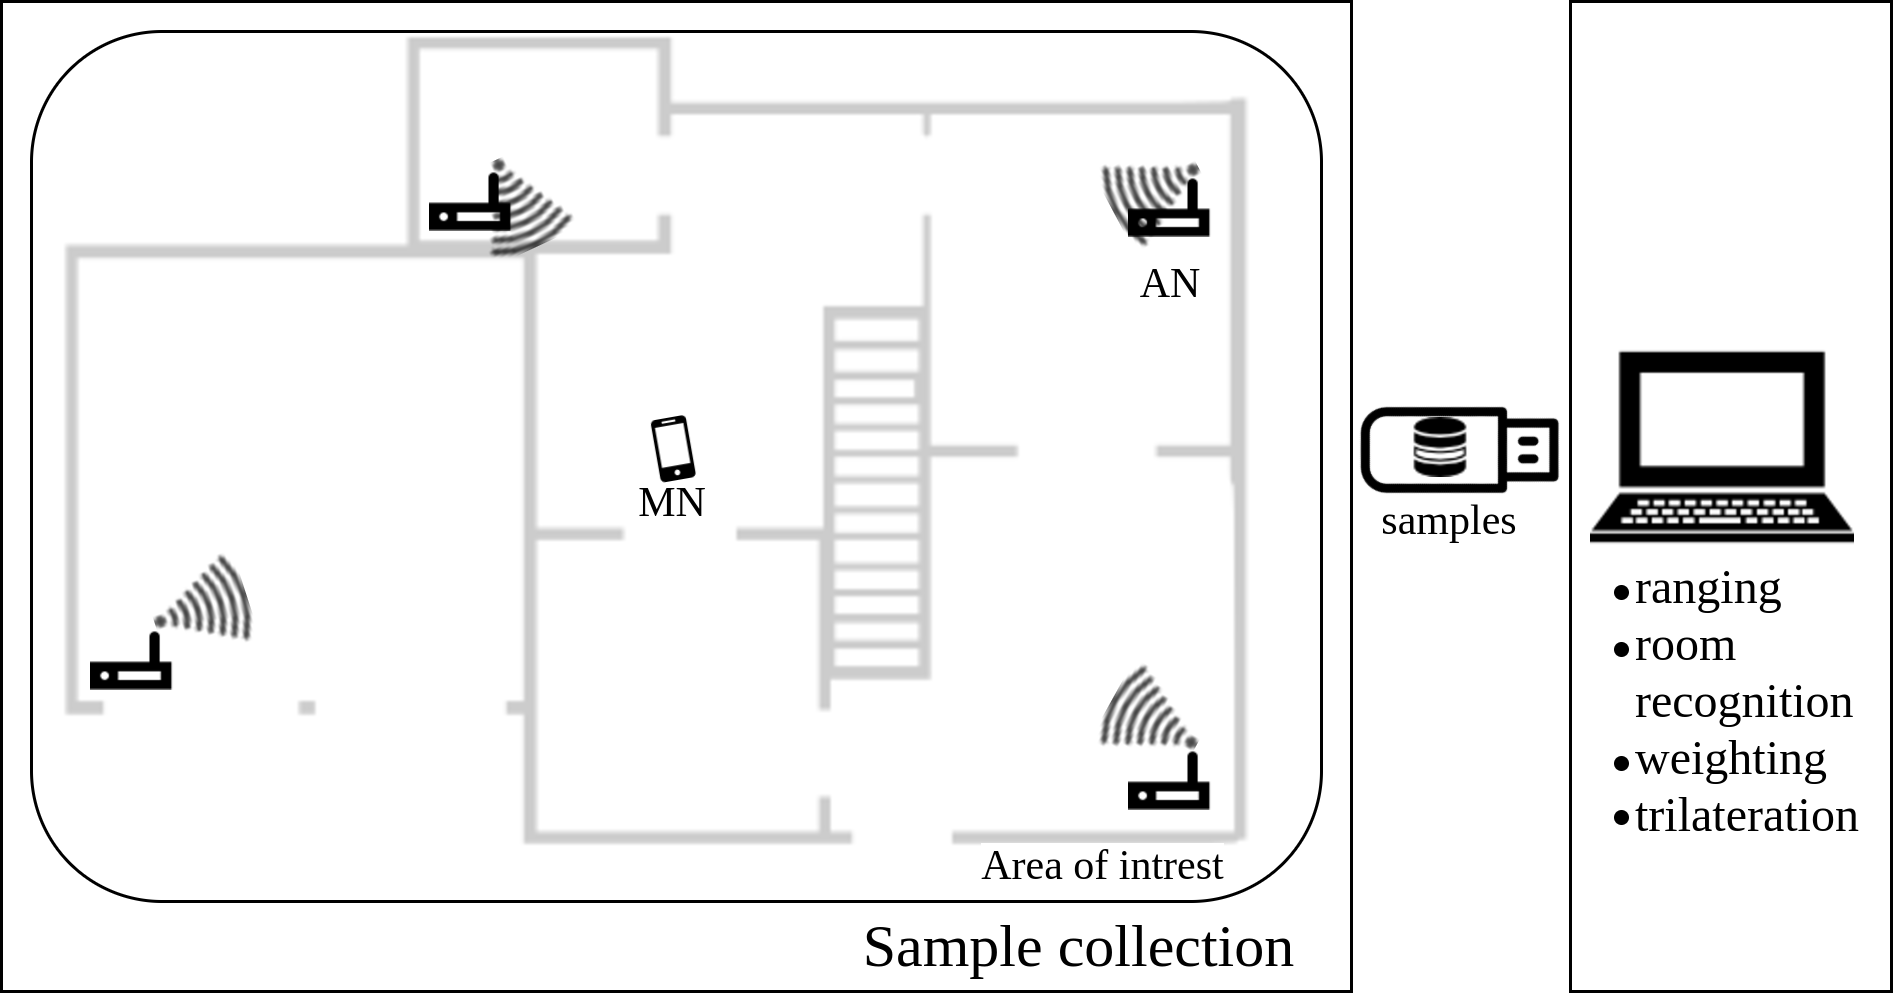
\includegraphics[width=\textwidth]{Figures/SystemImplementationOverview}
\decoRule
\caption[Test bed implementation overview]{Overview of the test bed implementation}
\label{fig:localizationSystemOverview}
\end{figure}

This test bed implementation splits the system into an online (collecting samples) and offline (calculations on the computer) part. This way it is possible to try out and empirically compare different configurations of the localisation system under the exact same conditions.

The set-up of this test bed comprises both hardware and software specific configurations for each component. The remainder of this chapter details these configurations.

\section{Hardware Set-up}

This set-up requires three different kinds of machines. One for the AN, another for the MN and a computer. There are no special requirements for the computer as long as it is able to execute Java code.

For the AN and MN the following hardware was employed:

\paragraph{Anchor Nodes}
The commercial Wi-Fi access points used as anchor nodes are of the model D-Link D-635 and D-2553. They are set-up with a beacon period of 100ms and broadcast on the 2.4 GHz frequency band.

\paragraph{Mobile Node}

The mobile node is an android smartphone of the model \emph{One Plus One}. It has the following specifications:

\begin{itemize}
\item \textbf{OS:} Android 5.1
\item \textbf{Processor:} 2.5GHz Quad-core CPU
\item \textbf{WiFi module:} Qualcomm WCN3680 802.11ac/FM/BT 4.0 Combo Chip 
\item \textbf{Internal sensors:} accelerometer, magnetometer, gyroscope, proximity, ambient light
\item \textbf{Memory:} 3 GB RAM
\end{itemize}

The WiFi module and the magnetometer are used for the sample collection. The magnetometer is reasonably accurate while the off-the-shelf WiFi interface is  prone to interferences.


\section{Software Set-up}

\subsection{Sample collection}

The samples are collected on the smartphone using a small application written for this purpose.

The samples consist of:
\begin{itemize}
\item \textbf{A label} eather indicating the room or the exact location where the sample was taken.
\item \textbf{A set of RSSI values}, one for each AN.
\item \textbf{The magnetic field strength} in \(\mu\)-Tesla along the devices x,y and z axis.
\end{itemize}

On android the WiFi module can not be accessed directly. Wi-Fi scans have to be initiated through the \code{AndroidAPI} and it only supports full scans\cite{brouwers2014incremental}. Full scans take longer so it is only possible to take one RSSI measurement every 1.5 seconds.

Due to the low sampling rate it is not practical to apply filters to remove noise from the $RSSI$. It is also not possible to access channel state information which could be used to mitigate some of the multipath effects.

To collect one sample the application takes the average of five RSSI and magnetometer measurements, each spaced 2 seconds apart. The samples are then saved to a \code{.csv} file on the smartphones internal storage and later transferred to the computer.

\subsection{Training and testing of the system}

Training, testing and evaluation of the localization system is done offline on a computer using Matlab, WEKA and a Java program for the trilateration.

First the collected samples are grouped into training and testing datasets and the ranging, room recognition and weighting models are generated from the training data.

Then the trilateration-tool reads the testing data, applies the models and solves the trilateration problem. It prints out the predicted position and the positioning error for each sample in the testing set.

\begin{figure}[ht]
\centering
\includegraphics[width=\textwidth]{Figures/Offline_Set-Up}
\decoRule
\caption[Test bed offline implementation]{Diagram of the offline implementation}
\label{fig:offlineImplementation}
\end{figure}

\subsubsection*{Room Recognition Model}
The SVM for the room recognition is trained in WEKA. It generates a multiclass SVM model from the training data set and may use grid search for the parameter selection. The training data set consists of samples containing RSSI \((RSSI_{i})\) and magnetic field \((B_{xyz})\) values labelled with the room number \((R\#)\).

\subsubsection*{Ranging Model}
For the ranging model the \(\alpha, \beta\) parameters from equation \ref{eqn:non-linear path loss model} need to be determined for each AN. This is done by fitting the equation to the testing data in \emph{Matlab}. The testing data set is a list of RSSI values and the corresponding distance \((D_{i})\) to the AN.

The resulting non-linear regression model is inaccurate with high RSSI values (samples verry close to the AN). To account for that the distances for these high values are set by hand.

\subsubsection*{Weighting Model}

The \emph{Room Weights} are calculated by hand based on equation \ref{eqn: Room Weights} in a spreadsheet program and imported into the trilateration tool.

The \emph{Distance Weights} are calculated by the trilateration tool during run time based on the equation \ref{eqn: distance weights}.

\subsubsection*{Testing}

The testing dataset contains samples with RSSI and magnetic field values and the position \((X,Y)\) where the sample was collected.

In a first step WEKA is used to predict the room number. The result is handed to the trilateration tool, which applies the ranging and weighting models to determine the predicted distances \((d_{i})\) and clculate the weights \((w_{i})\). It then solves the trilateration problem (equation \ref{eqn: trilateration as optimization problem}) using the Levenberg–Marquardt optimizer from the \code{Apache Commons Math} library. It outputs the predicted position \((x,y)\) and the localization error to a \code{.csv} file.